\documentclass[]{IEEEtran}
%\IEEEoverridecommandlockouts
% The preceding line is only needed to identify funding in the first footnote. If that is unneeded, please comment it out.
\usepackage{cite}

% Your packages go here
\usepackage[utf8]{inputenc}
\usepackage{romannum}
\usepackage{graphicx}
\usepackage{caption,subcaption}
\usepackage{listings}
\usepackage{color}
\usepackage{url}
\usepackage{amsmath}
\usepackage{nccmath}
\usepackage{mathtools}
\usepackage{hyperref}
\DeclarePairedDelimiter{\norm}{\lVert}{\rVert}

\definecolor{dkgreen}{rgb}{0,0.6,0}
\definecolor{gray}{rgb}{0.5,0.5,0.5}
\definecolor{mauve}{rgb}{0.58,0,0.82}

\lstset{frame=tb,
  language=python,
  aboveskip=3mm,
  belowskip=3mm,
  showstringspaces=false,
  columns=flexible,
  basicstyle={\small\ttfamily},
  numbers=none,
  numberstyle=\tiny\color{gray},
  keywordstyle=\color{blue},
  commentstyle=\color{dkgreen},
  stringstyle=\color{mauve},
  breaklines=true,
  breakatwhitespace=true,
  tabsize=3,
  literate={á}{{\'a}}1
           {ç}{{\c{c}}}1
           {ü}{{\"u}}1
           {é}{{\'e}}1
}

\def\BibTeX{{\rm B\kern-.05em{\sc i\kern-.025em b}\kern-.08em
    T\kern-.1667em\lower.7ex\hbox{E}\kern-.125emX}}

\markboth{MC949/MO446 Computer Vision - HW4}{}

\begin{document}
  \title{Interfaces from hand-drawn sketches}
  \author{Darley Barreto, Edgar Tanaka, Tiago Barros
    \thanks{228120, 023577, 093125}
  }
  \maketitle

  \begin{abstract}
    In this work, we present a method that reads a video of someone drawing a sketch of a user interface, detects and interprets blocks of text, headers, and images, and outputs a valid HTML document based on this sketch. We begin by discussing the building blocks of our process. Then, we show some results of experiments on different videos, each one with its qualitative difficulty. Finally, we discuss some of its problems and the choices we made that gave us the proposed process.

  \end{abstract}

  \section{Introduction}
    This work presents a three staged simple process, as illustrated in Figure \ref{process}, which shows the reading of a handwritten wireframe HTML mockup from a video and the generation of a valid HTML document. The process can be splitted in the following tasks:
    \begin{itemize}
    \item Detection of shapes in a given video frame using Suzuki and Abe \cite{suzuki85} method and Ramer–Douglas–Peucker algorithm (RDP, \cite{rdp}).
    \item Decision of whether a detected shape is valid or not.
    \item Generation of HTML document.
    \end{itemize}

   \begin{figure}[h]
   \centering
   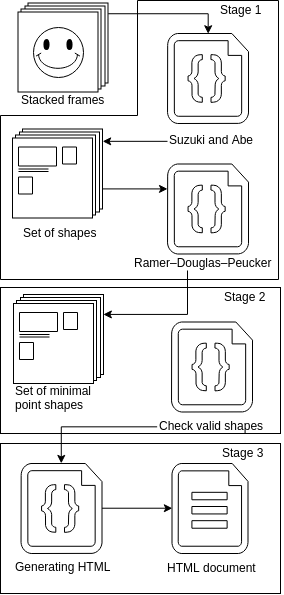
\includegraphics[width=0.25\textwidth]{figures/diagram.png}
   \caption{\label{process} Example of Ramer–Douglas–Peucker algorithm}
  \end{figure}

  Blablabla

  \section{Detection of shape patterns}
  In this stage, we discuss the detection of simple shapes as lines and rectangles. We begin by reading a video frame, then we resize the video to a fixed width of $300$ pixels and height of a value such that we are able to maintain the same aspect ratio as the original video. After resizing, we convert the frame to grayscale and apply a Gaussian Blur using a $5 \times 5$ kernel.

  After preprocessing the image into a more smooth one, we apply the Canny Edge Detector \cite{canny}, which gives us a binary image and we can detect contours using Suzuki and Abe method. This method retrieves contours from a binary image, and thus is a useful tool for shape analysis and object detection and recognition.

  In the original paper, the authors first present an algorithm which can extract the topological structure of a given binary image. This algorithm is an extended version of the border following algorithm, which discriminates between outer borders and hole borders. The extensions are: (1) to put a unique mark on each border rather than to adopt the same marking procedure for every border; and (2) to add a procedure for obtaining the parent border of the currently followed border. With this algorithm, they say that we can extract the surroundness relation among the borders, which corresponds to the surroundness relation among the connected components.

  If a binary image is stored in the form of the borders and the surroundness relation is extracted by this algorithm, some simple image processing can be done without restoring the original image. Thus, the method offers an effective way of storing binary image data. Next, they show a modified version of the first algorithm which follows only the outermost borders of a binary image (i.e., the outer borders which are not surrounded by holes). When we want to ignore the l-components which are surrounded by other l-components, this modified algorithm gives us a quick, sequential method of counting the l-components or shrinking each l-component to one point.

   \begin{figure}[h]
   \centering
   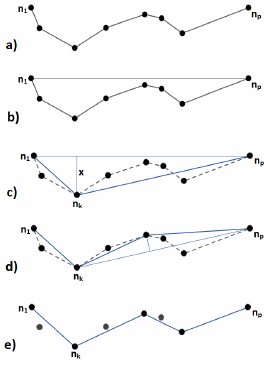
\includegraphics[width=0.25\textwidth]{figures/rdp.png}
   \caption{\label{rdp} Example of Ramer–Douglas–Peucker algorithm. Source: \href{https://www.researchgate.net/figure/Input-curve-specified-stages-of-the-Ramer-Douglas-Peucker-algorithm-output-curve-with_fig1_236024099}{Research Gate}.}
  \end{figure}

  For each possible shape found by the Suzuki and Abe's method, we want to reduce the points in the contour to the smaller set. The Ramer–Douglas–Peucker (RDP) algorithm (see Figure \ref{rdp}) is an algorithm for reducing the number of points in a curve that is approximated by a series of points.

  The input of the RDP algorithm is a curve represented by an ordered set of points $(P_1,\dots,P_n)$ and a threshold $\epsilon > 0$ . The output is the curve represented by a subset of the input set of points. On the first step of the algorithm, we search for the farthest point $(P_z)$ from the line segment between the start and the end points ($P_1$ and $P_n$). If that point is closer than the threshold $(\epsilon)$, all the points between $P_1$ and $P_n$ are discarded. Otherwise, $P_z$ is included in the resulting set. Then, we repeat the same step recursively with the right and the left parts of the curve (from $P_1$ to $P_z$ and from $P_z$ to $P_n$). Then, we merge the results of processing the left and the right parts. The algorithm repeats until all the points are handled.

  In this manner, shapes similar to a rectangle, but that may have more than $4$ points can be approximated by RDP in a $4$ point version. Contour approximation is predicated on the assumption that a curve can be approximated by a series of short line segments. This leads to a resulting approximated curve that consists of a subset of points that were defined by the original curve \cite{shape_detection}.

  After the RDP, we have a set of possible shapes and their approximated points. We search for shapes that have $2$ or $4$ points, that is, a line or a rectangle respectively. Once we retrieve the matches, we send the shapes to the next stage to decide whether to pick a shape or not.

  \section{Elements model from shape patterns}
  Using the detection of shape patterns described in the previous section, we can detect lines and rectangles. Every detected rectangle in the sketch represents an image in the layout. When it comes to lines, they could represent both headers and lines of text. To differentiate between them, we use the computed contour by Suzuki and Abe's method to calculate the area and the perimeter of the line contour. If the ratio $\frac{area}{perimeter} >= 2.0$, then we treat the line as a header, otherwise we treat it as text line.

  The reasoning behind this method, which is a heuristic in fact, is that headers are represented by a thick line, as per Figure~1 of the project description document, while text lines are represented by thinner lines. Moreover, headers and text lines could span any arbitrary width. To make our solution more robust, we cannot simply consider the line height in pixels, as this would clearly only work in some circumstances. So, we thought of using the ratio of the area of the line and its perimeter, as this produces a number without a unit of measurement, meaning that it should work reasonably well irrespective of the size of the video frame. Also, it accounts for the fact that the line could be long or short, because both the area and the perimeter grow when the line is longer, and both shrink when the line is shorter.

  Considering that this method is a heuristic, it is not guaranteed to work in every possible scenario. But it worked well on every sketch that it was tested on, provided that the Canny Edge Detector identified correctly the borders of the line, which sometimes it does not, as discussed in section~\ref{sec:discussion}.

  If a line is considered to represent a line of text, it is placed in a text block. If it is the first line of text detected, a new text block is created for it, otherwise we compute the distance between this line and every text block, and when/if we find a text block close enough, then we append this line of text into that text block. If there is no text block close enough, then we create a new one for the line. But what does ``close enough'' mean? In this case, we use the euclidean distance between the top left corner of the bounding box of the line of text being considered and the top left (first) and the bottom left (second) corner of the bounding box of the text block (see Figure~\ref{fig:detection} for a depiction of bounding boxes, in red). If the distance is less than a threshold (set as 70 as its default value), then the line and the text block are considered to be close enough, otherwise they are not.

  \begin{figure}[h]
    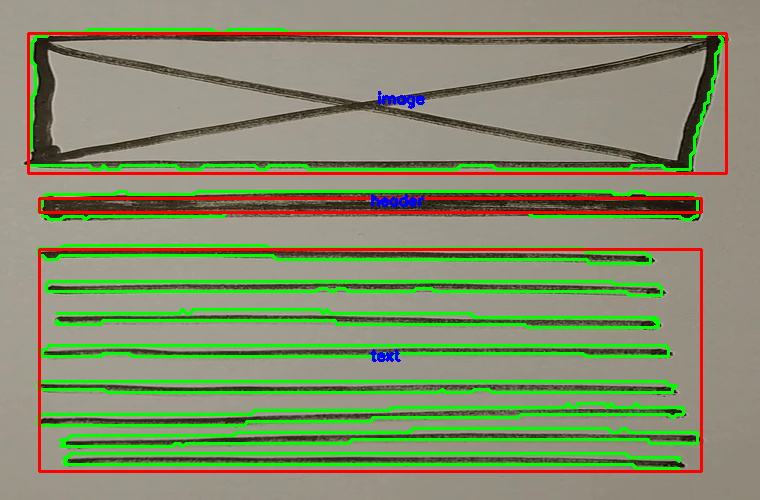
\includegraphics[width=\linewidth]{./figures/detection.png}
    \caption{Elements detected in a sample sketch.}
    \label{fig:detection}
  \end{figure}

  An example of the visual representation of the underlying elements model is shown in Figure~\ref{fig:detection}. The green lines are the contour as detected by Suzuki and Abe's method. The red rectangles are the bounding boxes of the detected elements, and written in blue are the types of the elements.

  \section{Generation of HTML from elements model}
  Gimme that layout, baby.

  \section{Discussion}
  \label{sec:discussion}
  In order to detect the shapes, firstly we resized the frames, converted them to grayscale and applied a Gaussian Blur, but instead of using the Canny Edge Detector we tried a simpler approach by taking threshold of each frame. The main problem with it was the noise introduced, some of the frames the chosen threshold introduced smaller black shapes into the frames in such way that the Suzuki and Abe's algorithm was not found properly the contours, and therefore the RDP algorithm was not working properly.

  The second main problem when using the threshold was that for some frames particular values yielded a good set of shape, that is, our pipeline was able to find the correct shapes, but for some frames, the threshold values gave a bad set of shapes. So we would have to check the threshold values for each frame of each video, which is not a good way of doing it.

  We tested the Canny algorithm because it can detect edges in salient regions, and we can use the results in the Suzuki and  Abe's algorithm. The frames have a great number of salient regions, once they are similar in structure: dark draws on a clear surface. After some tests, we found a set of possible values of the parameters for the algorithm that gave good qualitative results on the videos tested. Unlike the treshold approach, we could use the same values for each frame and each video without any major loss.

  \section{Conclusion}
  Can I conclude the semester already?

  \begin{thebibliography}{00}
    \bibitem{shape_detection} Rosebrock, A. (2016). ``OpenCV shape detection''. Site visited on November 13, 2018, from \url{https://www.pyimagesearch.com/2016/02/08/opencv-shape-detection/}
    \bibitem{suzuki85} Suzuki, S. (1985). ``Topological structural analysis of digitized binary images by border following''. Computer vision, graphics, and image processing, 30(1), 32-46.
    \bibitem{canny} Canny, J. (1986). ``A computational approach to edge detection''. IEEE Transactions on pattern analysis and machine intelligence, (6), 679-698.
    \bibitem{rdp} Douglas, D. H., \& Peucker, T. K. (1973). ``Algorithms for the reduction of the number of points required to represent a digitized line or its caricature''. Cartographica: The International Journal for Geographic Information and Geovisualization, 10(2), 112-122.
  \end{thebibliography}
\end{document}
